\documentclass[12pt,twoside]{memoir}

\usepackage{libertine}
\usepackage[T1,LGR]{fontenc}
\usepackage{titlesec, xcolor}
\usepackage[utf8]{inputenc}
\usepackage[greek.ancient]{babel}
\usepackage{lettrine}
\usepackage{graphicx}

%for chapter headings
\definecolor{gray75}{gray}{0.75}
\newcommand{\hsp}{\hspace{20pt}} 
\titleformat{\chapter}[hang]{\Huge\bfseries}{\thechapter\hsp\textcolor{gray75}{|}\hsp}{0pt}{\Huge\bfseries}

%eliminate widows and orphans
\widowpenalty=10000
\clubpenalty=10000

\newcommand{\bibleref}[2]{\selectlanguage{english}\textbf{#1} \selectlanguage{greek}{#2}}
\newcommand{\biblefoot}[2]{\footnote{\bibleref{#1}{#2}}}
\newcommand{\biblefootduo}[4]{\footnote{\bibleref{#1}{#2}\ldots \bibleref{#3}{#4}}}
\newcommand{\biblefoottrio}[6]{\footnote{\bibleref{#1}{#2}\ldots \bibleref{#3}{#4}\ldots \bibleref{#5}{#6}}}
\newcommand{\biblefootcuarto}[8]{\footnote{\bibleref{#1}{#2}\ldots \bibleref{#3}{#4}\ldots \bibleref{#5}{#6}\ldots \bibleref{#7}{#8}}}

%title	
%% publisher’s logo
\providecommand{\HUGE}{\Huge}
\newlength{\drop}
\newcommand*{\titleGM}{\begingroup% Gentle Madness
\drop = 0.1\textheight
\vspace{\baselineskip}
\vfill
	\hbox{%
	\hspace*{0.2\textwidth}%
	\rule{1pt}{\textheight}
	\hspace*{0.05\textwidth}%
	\parbox[b]{0.75\textwidth}{
	\vbox{%
		\vspace{\drop}
		{\noindent\HUGE\bfseries\textcolor{red}{\begin{foreignlanguage}{english}{The Revelation}\end{foreignlanguage}}\\[0.5\baselineskip]\textcolor{red}{\begin{foreignlanguage}{english}{of Jesus Christ}\end{foreignlanguage}}\\\\}
		{\Large\itshape \begin{foreignlanguage}{english}{Reading in Light of the Shadows\end{foreignlanguage}}}\\[4\baselineskip]		
		{\noindent \begin{foreignlanguage}{english}{Arranged by Caleb George\end{foreignlanguage}}}\par
		\vspace{0.4\textheight}
		{\textbf{\begin{foreignlanguage}{english}{Kephali Press\end{foreignlanguage}}}}\\[\baselineskip]
		}% end of vbox
		}% end of parbox
	}% end of hbox
\vfill
\endgroup}

%figure captions
\addto\captionsgreek{\renewcommand{\figurename}{\begin{foreignlanguage}{english}{Fig.}\end{foreignlanguage}}}

%verse numbers
\newcommand{\vnum}[1]{\textcolor{red}{\Large{#1}}}

\begin{document}
\pagestyle{empty}
\titleGM

\begin{figure*}[p!]
	\centering
       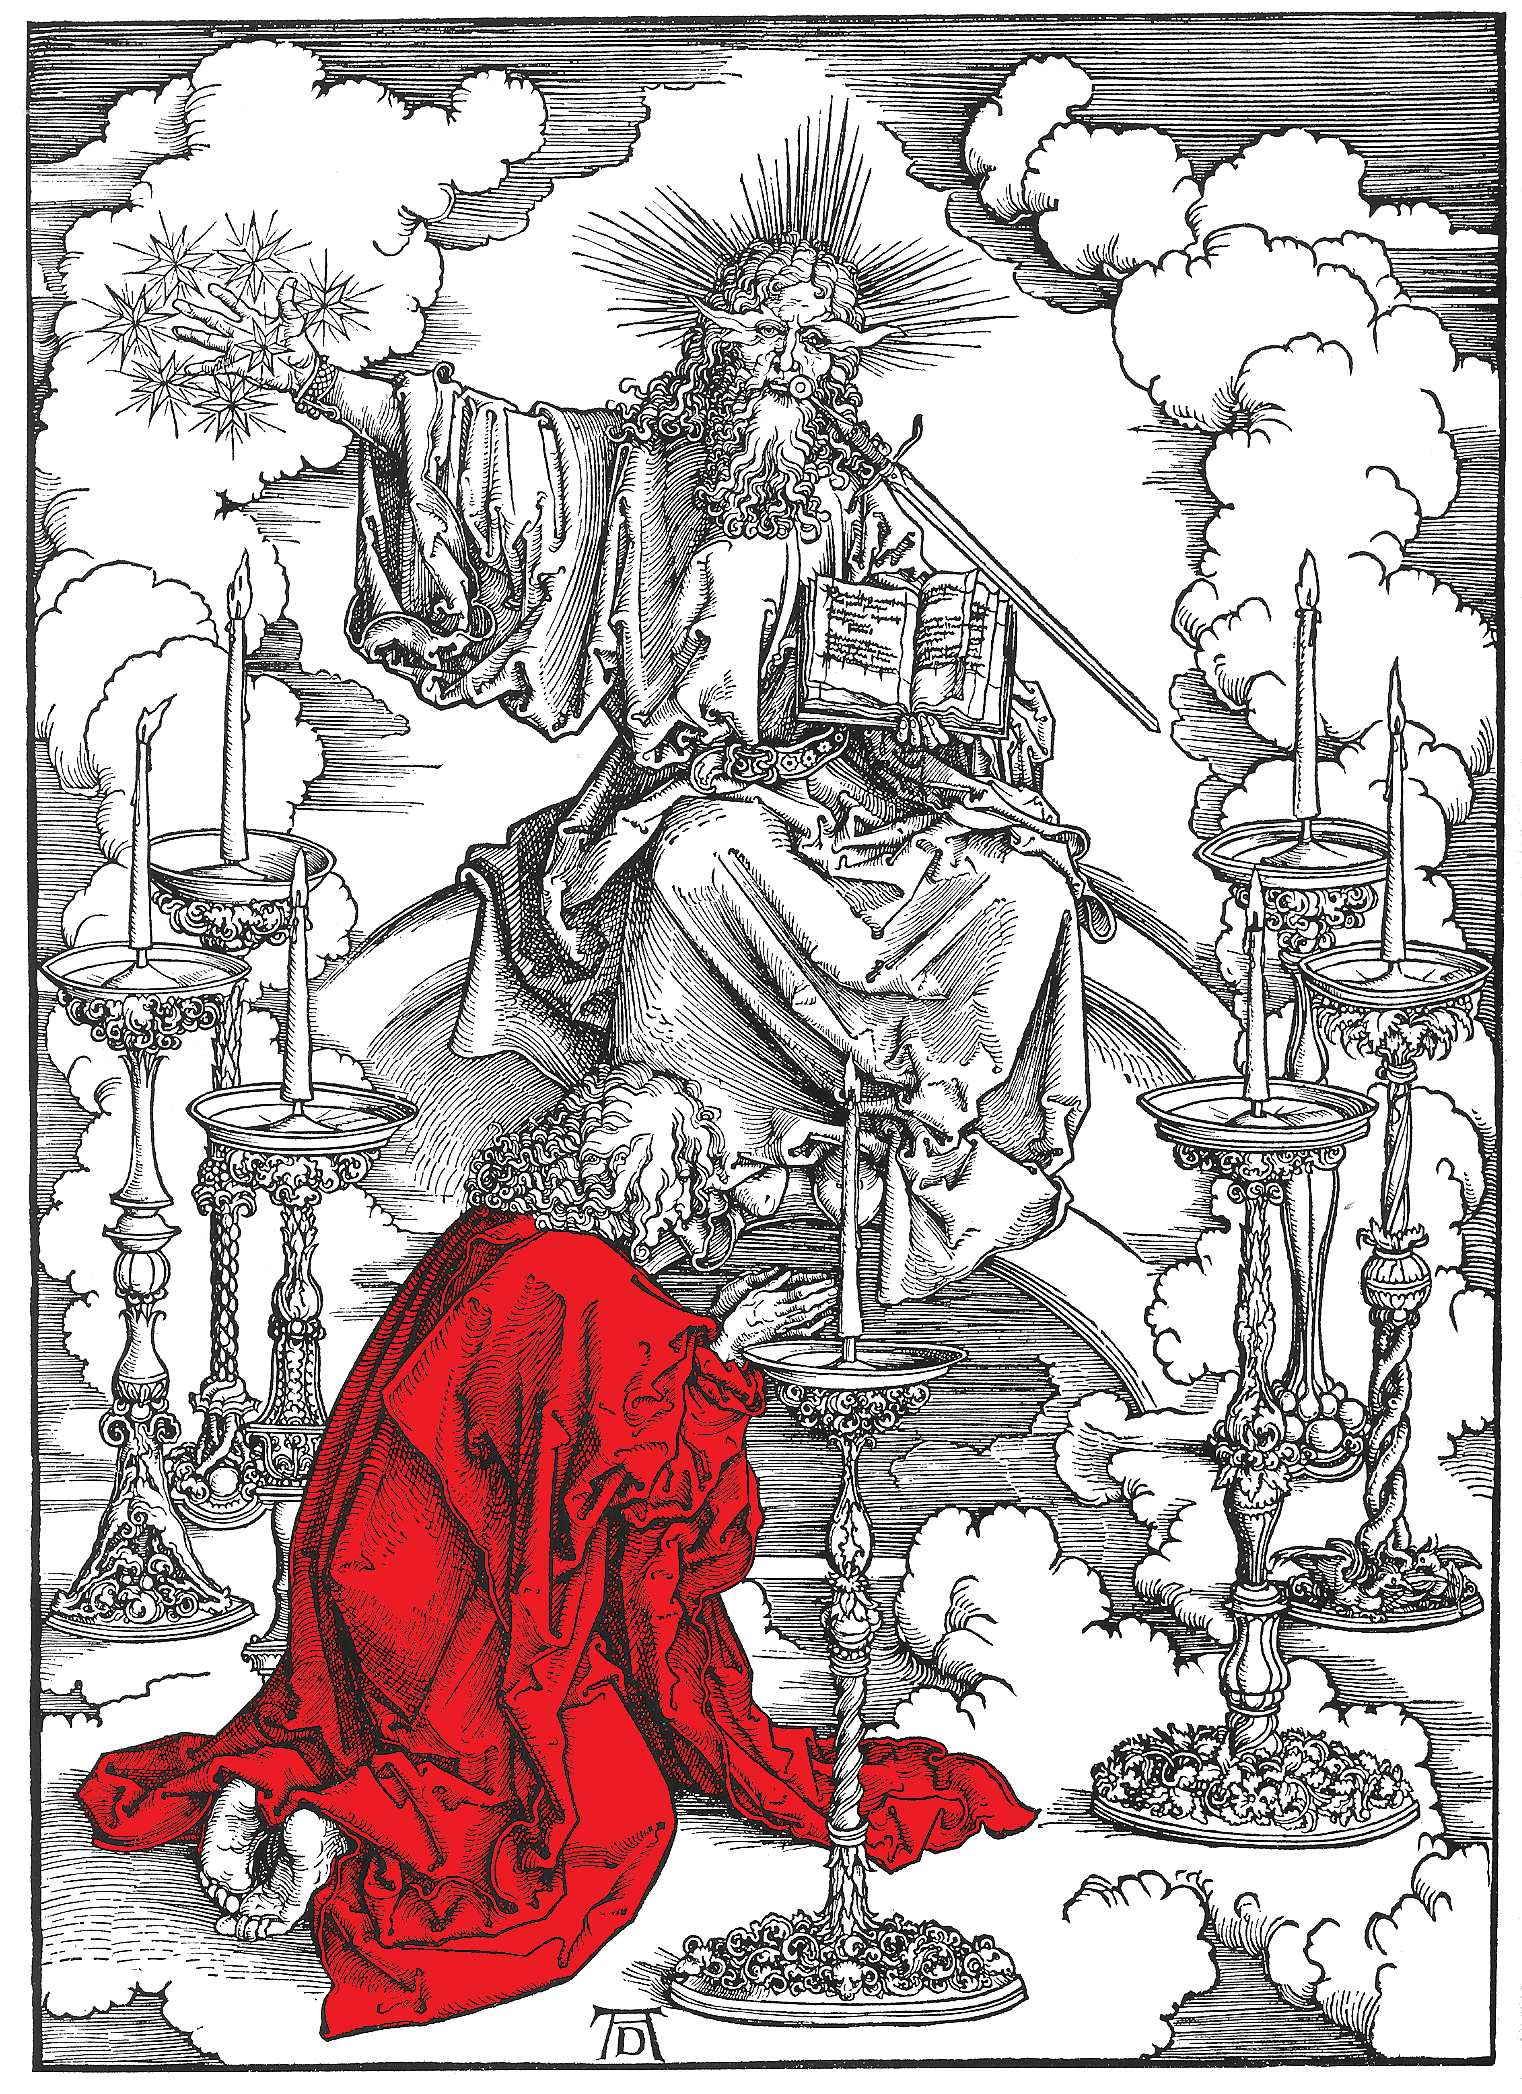
\includegraphics[scale=0.3]{Durer/Durer-candlesticks.png}    
    	\caption{\begin{foreignlanguage}{english}{St. John's Vision of the Seven Candlesticks. Albrecht Dürer, 1498.}\end{foreignlanguage}}
    	\label{fig:candlesticks}
\end{figure*}
\clearpage

\mainmatter
\fontfamily{Linux Libertine O}\selectfont
\lettrine[lines=4]{\textcolor{red}{A}}{}ποκaλυψις%
	\biblefootduo{Dan 2.28}{ἀλλ᾽ ἔστι θεὸς ἐν οὐρανῷ ἀνακαλύπτων μυστήρια}%
					{Amos 3.7}{διότι οὐ μὴ ποιήσῃ κύριος ὁ θεὸς πρᾶγμα, ἐὰν μὴ ἀποκαλύψῃ παιδείαν αὐτοῦ πρὸς τοὺς δούλους αὐτοῦ τοὺς προφήτας} %
Ἰησοῦ Χριστοῦ ἣν ἔδωκεν αὐτῷ ὁ θεὸς δεῖξαι τοῖς δούλοις αὐτοῦ ἃ δεῖ γενέσθαι ἐν τάχει, καὶ ἐσήμανεν ἀποστείλας διὰ τοῦ ἀγγέλου αὐτοῦ τῷ δούλῳ αὐτοῦ Ἰωάννῃ, \vnum{2} ὃς ἐμαρτύρησεν τὸν λόγον τοῦ θεοῦ καὶ τὴν μαρτυρίαν Ἰησοῦ Χριστοῦ ὅσα εἶδεν. \vnum{3} Μακάριος ὁ ἀναγινώσκων καὶ οἱ ἀκούοντες τοὺς λόγους τῆς προφητείας καὶ τηροῦντες τὰ ἐν αὐτῇ γεγραμμένα, ὁ γὰρ καιρὸς ἐγγύς.

\vnum{4} Ἰωάννης ταῖς ἑπτὰ ἐκκλησίαις ταῖς ἐν τῇ Ἀσίᾳ· χάρις ὑμῖν καὶ εἰρήνη ἀπὸ ὁ ὢν\biblefoot{Ex 3.14}{εἶπεν ὁ θεὸς πρὸς Μωυσῆν ᾿Εγώ εἰμι ὁ ὤν} καὶ ὁ ἦν καὶ ὁ ἐρχόμενος καὶ ἀπὸ τῶν ἑπτὰ πνευμάτων\biblefoot{Is 11.2-3}{ἀναπαύσεται ἐπ᾽ αὐτὸν πνεῦμα τοῦ θεοῦ, πνεῦμα σοφίας καὶ συνέσεως, πνεῦμα βουλῆς καὶ ἰσχύος, πνεῦμα γνώσεως καὶ εὐσεβείας· ἐμπλήσει αὐτὸν πνεῦμα φόβου θεοῦ} ἃ ἐνώπιον τοῦ θρόνου αὐτοῦ \vnum{5} καὶ ἀπὸ Ἰησοῦ Χριστοῦ, ὁ μάρτυς, ὁ πιστός, ὁ πρωτότοκος\biblefoot{Ps 88(87).28}{κἀγὼ πρωτότοκον θήσομαι αὐτόν, ὑψηλὸν παρὰ τοῖς βασιλεῦσιν τῆς γῆς} τῶν νεκρῶν καὶ ὁ ἄρχων τῶν βασιλέων τῆς γῆς%
	\biblefoot{Dan 7.14}{καὶ ἐδόθη αὐτῷ ἐξουσία, καὶ πάντα τὰ ἔθνη τῆς γῆς κατὰ γένη καὶ πᾶσα δόξα αὐτῷ λατρεύουσα· καὶ ἡ ἐξουσία αὐτοῦ ἐξουσία αἰώνιος, ἥτις οὐ μὴ ἀρθῇ, καὶ ἡ βασιλεία αὐτοῦ, ἥτις οὐ μὴ φθαρῇ}%
. Τῷ ἀγαπῶντι ἡμᾶς%
	\biblefootduo{Deut 7.8}{ἀλλὰ παρὰ τὸ ἀγαπᾶν κύριον ὑμᾶς\ldots ἐξήγαγεν κύριος ὑμᾶς ἐν χειρὶ κραταιᾷ καὶ ἐν βραχίονι ὑψηλῷ καὶ ἐλυτρώσατο ἐξ οἴκου δουλείας ἐκ χειρὸς Φαραω βασιλέως Αἰγύπτου}%
				{23.6}{μετέστρεψεν κύριος ὁ θεός σου τὰς κατάρας εἰς εὐλογίαν, ὅτι ἠγάπησέν σε κύριος ὁ θεός σου} %
καὶ λύσαντι ἡμᾶς ἐκ τῶν ἁμαρτιῶν ἡμῶν ἐν τῷ αἵματι αὐτοῦ, %
\vnum{6} καὶ ἐποίησεν ἡμᾶς βασιλείαν, ἱερεῖς%
	\biblefootduo{Ex 19.6}{ὑμεῖς δὲ ἔσεσθέ μοι βασίλειον ἱεράτευμα καὶ ἔθνος ἅγιον}%
				{Is 61.6}{ὑμεῖς δὲ ἱερεῖς κυρίου κληθήσεσθε, λειτουργοὶ θεοῦ} %
τῷ θεῷ καὶ πατρὶ αὐτοῦ, αὐτῷ ἡ δόξα καὶ τὸ κράτος εἰς τοὺς αἰῶνας [τῶν αἰώνων]· ἀμήν%
	\biblefoot{Ps 71(70).18-19}{Εὐλογητὸς κύριος ὁ θεὸς\ldots καὶ εὐλογητὸν τὸ ὄνομα τῆς δόξης αὐτοῦ εἰς τὸν αἰῶνα καὶ εἰς τὸν αἰῶνα τοῦ αἰῶνος, καὶ πληρωθήσεται τῆς δόξης αὐτοῦ πᾶσα ἡ γῆ. γένοιτο γένοιτο.}%
.
\begin{verse}
\vnum{7} Ἰδοὺ ἔρχεται μετὰ τῶν νεφελῶν%
	\biblefootcuarto{Ps 96.2}{νεφέλη καὶ γνόφος κύκλῳ αὐτοῦ}%
				{Is 19.1}{᾿Ιδοὺ κύριος κάθηται ἐπὶ νεφέλης κούφης καὶ ἥξει εἰς Αἴγυπτον}%
				{Dan 7.13}{ἰδοὺ ἐπὶ τῶν νεφελῶν τοῦ οὐρανοῦ ὡς υἱὸς ἀνθρώπου ἤρχετο}%
				{Na 1.3}{κύριος μακρόθυμος, καὶ μεγάλη ἡ ἰσχὺς αὐτοῦ\ldots ἐν συντελείᾳ καὶ ἐν συσσεισμῷ ἡ ὁδὸς αὐτοῦ, καὶ νεφέλαι κονιορτὸς ποδῶν αὐτοῦ}%
,\\
καὶ ὄψεται αὐτὸν πᾶς ὀφθαλμὸς\\
καὶ οἵτινες αὐτὸν ἐξεκέντησαν,\\
καὶ κόψονται ἐπ’ αὐτὸν πᾶσαι αἱ φυλαὶ τῆς γῆς%
	\biblefoot{Zech 12.10-14}{καὶ ἐπιβλέψονται πρός με ἀνθ᾽ ὧν κατωρχήσαντο [\selectlanguage{english}Aquila, Theototion: \selectlanguage{greek}ἐξεκέντησαν;\selectlanguage{english} cf. Jn 19.37\selectlanguage{greek}] καὶ κόψονται ἐπ᾽ αὐτὸν κοπετὸν ὡς ἐπ᾽ ἀγαπητὸν καὶ ὀδυνηθήσονται ὀδύνην ὡς ἐπὶ πρωτοτόκῳ. ἐν τῇ ἡμέρᾳ ἐκείνῃ μεγαλυνθήσεται ὁ κοπετὸς ἐν Ιερουσαλημ ὡς κοπετὸς ῥοῶνος ἐν πεδίῳ ἐκκοπτομένου, καὶ κόψεται ἡ γῆ κατὰ φυλὰς φυλάς\ldots}. 
\end{verse}

ναί, ἀμήν.

\vnum{8} Ἐγώ εἰμι τὸ ἄλφα καὶ τὸ ὦ%
	\biblefootcuarto{Is 41.4}{ἐγὼ θεὸς πρῶτος, καὶ εἰς τὰ ἐπερχόμενα ἐγώ εἰμι}%
	{43.10}{ἐγώ εἰμι, ἔμπροσθέν μου οὐκ ἐγένετο ἄλλος θεὸς καὶ μετ᾽ ἐμὲ οὐκ ἔσται}%
	{44.6}{᾿Εγὼ πρῶτος καὶ ἐγὼ μετὰ ταῦτα, πλὴν ἐμοῦ οὐκ ἔστιν θεός}%
	{48.12}{ἐγώ εἰμι πρῶτος, καὶ ἐγώ εἰμι εἰς τὸν αἰῶνα}%
, λέγει κύριος ὁ θεός, ὁ ὢν%
	\footnote{\selectlanguage{english}cf. v 4\selectlanguage{greek}} %
καὶ ὁ ἦν καὶ ὁ ἐρχόμενος, ὁ παντοκράτωρ.

\vnum{9} Ἐγὼ Ἰωάννης, ὁ ἀδελφὸς ὑμῶν καὶ συγκοινωνὸς ἐν τῇ θλίψει καὶ βασιλείᾳ καὶ ὑπομονῇ ἐν Ἰησοῦ, ἐγενόμην ἐν τῇ νήσῳ τῇ καλουμένῃ Πάτμῳ διὰ τὸν λόγον τοῦ θεοῦ καὶ τὴν μαρτυρίαν Ἰησοῦ %
\vnum{10} ἐγενόμην ἐν πνεύματι ἐν τῇ κυριακῇ ἡμέρᾳ καὶ ἤκουσα ὀπίσω μου φωνὴν μεγάλην ὡς σάλπιγγος %
\vnum{11} λεγούσης· ὃ βλέπεις γράψον εἰς βιβλίον%
	\biblefoottrio{Is 30.8}{Νῦν οὖν καθίσας γράψον ἐπὶ πυξίου ταῦτα καὶ εἰς βιβλίον, ὅτι ἔσται εἰς ἡμέρας καιρῶν ταῦτα καὶ ἕως εἰς τὸν αἰῶνα}%
				{Jer 37(30).2}{Οὕτως εἶπεν κύριος ὁ θεὸς Ισραηλ λέγων Γράψον πάντας τοὺς λόγους, οὓς ἐχρημάτισα πρὸς σέ, ἐπὶ βιβλίου}%
				{Hab 2.2}{καὶ ἀπεκρίθη πρός με κύριος καὶ εἶπεν Γράψον ὅρασιν καὶ σαφῶς ἐπὶ πυξίον, ὅπως διώκῃ ὁ ἀναγινώσκων αὐτά} %
καὶ πέμψον ταῖς ἑπτὰ ἐκκλησίαις, εἰς Ἔφεσον καὶ εἰς Σμύρναν καὶ εἰς Πέργαμον καὶ εἰς Θυάτειρα καὶ εἰς Σάρδεις καὶ εἰς Φιλαδέλφειαν καὶ εἰς Λαοδίκειαν.

\vnum{12} Καὶ ἐπέστρεψα βλέπειν τὴν φωνὴν ἥτις ἐλάλει μετ’ ἐμοῦ, καὶ ἐπιστρέψας εἶδον ἑπτὰ λυχνίας χρυσᾶς%
	\biblefootduo{Ex 25.37}{καὶ ποιήσεις τοὺς λύχνους αὐτῆς ἑπτά· καὶ ἐπιθήσεις τοὺς λύχνους, καὶ φανοῦσιν ἐκ τοῦ ἑνὸς προσώπου}%
	{Zech 4.2}{καὶ εἶπεν πρός με Τί σὺ βλέπεις; καὶ εἶπα ῾Εώρακα καὶ ἰδοὺ λυχνία χρυσῆ ὅλη, καὶ τὸ λαμπαδεῖον ἐπάνω αὐτῆς, καὶ ἑπτὰ λύχνοι ἐπάνω αὐτῆς, καὶ ἑπτὰ ἐπαρυστρίδες τοῖς λύχνοις τοῖς ἐπάνω αὐτῆς} %
\vnum{13} καὶ ἐν μέσῳ τῶν λυχνιῶν ὅμοιον υἱὸν ἀνθρώπου%
	\biblefoottrio{Ez 1.26}{καὶ ἐπὶ τοῦ ὁμοιώματος τοῦ θρόνου ὁμοίωμα ὡς εἶδος ἀνθρώπου ἄνωθεν}%
			{Dan 7.13}{ἐθεώρουν ἐν ὁράματι τῆς νυκτὸς καὶ ἰδοὺ ἐπὶ τῶν νεφελῶν τοῦ οὐρανοῦ ὡς υἱὸς ἀνθρώπου ἤρχετο, καὶ ὡς παλαιὸς ἡμερῶν παρῆν, καὶ οἱ παρεστηκότες παρῆσαν αὐτῷ.}%
			{Dan 10.16}{καὶ ἰδοὺ ὡς ὁμοίωσις χειρὸς ἀνθρώπου\ldots}
ἐνδεδυμένον ποδήρη%
	\biblefoot{Dan 7.9}{\ldots ἔχων περιβολὴν ὡσεὶ χιόνα}% 
καὶ περιεζωσμένον πρὸς τοῖς μαστοῖς ζώνην χρυσᾶν%
	\biblefoot{Dan 10.5}{καὶ ἦρα τοὺς ὀφθαλμούς μου καὶ εἶδον καὶ ἰδοὺ ἄνθρωπος εἷς ἐνδεδυμένος βύσσινα καὶ τὴν ὀσφὺν περιεζωσμένος βυσσίνῳ, καὶ ἐκ μέσου αὐτοῦ φῶς}%
. \vnum{14} ἡ δὲ κεφαλὴ αὐτοῦ καὶ αἱ τρίχες λευκαὶ ὡς ἔριον λευκὸν ὡς χιὼν%
	\biblefoot{Dan 7.9}{καὶ παλαιὸς ἡμερῶν ἐκάθητο\ldots καὶ τὸ τρίχωμα τῆς κεφαλῆς αὐτοῦ ὡσεὶ ἔριον λευκὸν καθαρόν}%
καὶ οἱ ὀφθαλμοὶ αὐτοῦ ὡς φλὸξ πυρὸς%
	\biblefoot{Dan 10.6}{καὶ τὸ πρόσωπον αὐτοῦ ὡσεὶ ὅρασις ἀστραπῆς, καὶ οἱ ὀφθαλμοὶ αὐτοῦ ὡσεὶ λαμπάδες πυρός} %
\vnum{15} καὶ οἱ πόδες αὐτοῦ ὅμοιοι χαλκολιβάνῳ ὡς ἐν καμίνῳ πεπυρωμένης%
	\biblefootduo{Ez 1.7}{καὶ πτερωτοὶ οἱ πόδες αὐτῶν, καὶ σπινθῆρες ὡς ἐξαστράπτων χαλκός}%
			{1.27}{καὶ εἶδον ὡς ὄψιν ἠλέκτρου ἀπὸ ὁράσεως ὀσφύος καὶ ἐπάνω, καὶ ἀπὸ ὁράσεως ὀσφύος καὶ ἕως κάτω εἶδον ὡς ὅρασιν πυρὸς καὶ τὸ φέγγος αὐτοῦ κύκλῳ} %	
καὶ ἡ φωνὴ αὐτοῦ ὡς φωνὴ ὑδάτων πολλῶν%
	\biblefootduo{Ps 92.4}{ἀπὸ φωνῶν ὑδάτων πολλῶν θαυμαστοὶ οἱ μετεωρισμοὶ τῆς θαλάσσης, θαυμαστὸς ἐν ὑψηλοῖς ὁ κύριος}%
        {Ez 1.24}{καὶ ἤκουον τὴν φωνὴν τῶν πτερύγων αὐτῶν ἐν τῷ πορεύεσθαι αὐτὰ ὡς φωνὴν ὕδατος πολλοῦ}%
, \vnum{16} καὶ ἔχων ἐν τῇ δεξιᾷ χειρὶ αὐτοῦ ἀστέρας ἑπτὰ καὶ ἐκ τοῦ στόματος αὐτοῦ ῥομφαία δίστομος ὀξεῖα ἐκπορευομένη%
	\biblefootduo{Is 11.4}{καὶ πατάξει γῆν τῷ λόγῳ τοῦ στόματος αὐτοῦ καὶ ἐν πνεύματι διὰ χειλέων ἀνελεῖ ἀσεβῆ}%
				{49.2}{καὶ ἔθηκεν τὸ στόμα μου ὡσεὶ μάχαιραν ὀξεῖαν} %
καὶ ἡ ὄψις αὐτοῦ ὡς ὁ ἥλιος φαίνει ἐν τῇ δυνάμει αὐτοῦ%
	\biblefootduo	{Is 60.19-20}{καὶ οὐκ ἔσται σοι ὁ ἥλιος εἰς φῶς ἡμέρας, οὐδὲ ἀνατολὴ σελήνης φωτιεῖ σοι τὴν νύκτα, ἀλλ᾽ ἔσται σοι κύριος φῶς αἰώνιον καὶ ὁ θεὸς δόξα σου. οὐ γὰρ δύσεται ὁ ἥλιός σοι, καὶ ἡ σελήνη σοι οὐκ ἐκλείψει· ἔσται γὰρ κύριός σοι φῶς αἰώνιον, καὶ ἀναπληρωθήσονται αἱ ἡμέραι τοῦ πένθους σου}%
			{Mal 4.2}{καὶ ἀνατελεῖ ὑμῖν τοῖς φοβουμένοις τὸ ὄνομά μου ἥλιος δικαιοσύνης}%
.

\vnum{17} Καὶ ὅτε εἶδον αὐτόν, ἔπεσα πρὸς τοὺς πόδας αὐτοῦ ὡς νεκρός
	\biblefootcuarto{Ez 1.28}{αὕτη ἡ ὅρασις ὁμοιώματος δόξης κυρίου· καὶ εἶδον καὶ πίπτω ἐπὶ πρόσωπόν μου}%
				{Dan 8.18}{καὶ λαλοῦντος αὐτοῦ μετ᾽ ἐμοῦ ἐκοιμήθην ἐπὶ πρόσωπον χαμαί}%
				{10.8-9}{καὶ ἐγὼ κατελείφθην μόνος καὶ εἶδον τὴν ὅρασιν τὴν μεγάλην ταύτην, καὶ οὐκ ἐ[γ]κατελείφθη ἐν ἐμοὶ ἰσχύς, καὶ ἰδοὺ πνεῦμα ἐπεστράφη ἐπ᾽ ἐμὲ εἰς φθοράν, καὶ οὐ κατίσχυσα. καὶ οὐκ ἤκουσα τὴν φωνὴν λαλιᾶς αὐτοῦ, ἐγὼ ἤμην πεπτωκὼς ἐπὶ πρόσωπόν μου ἐπὶ τὴν γῆν}%
				{10.17}{καὶ ἐγὼ ἠσθένησα, καὶ οὐκ ἔστιν ἐν ἐμοὶ ἰσχύς, καὶ πνεῦμα οὐ κατελείφθη ἐν ἐμοί}%
, καὶ ἔθηκεν τὴν δεξιὰν αὐτοῦ ἐπ’ ἐμὲ%
	\biblefootduo{Dan 8.18}{καὶ ἁψάμενός μου ἤγειρέ με ἐπὶ τοῦ τόπου}%
				{10.10}{καὶ ἰδοὺ χεῖρα προσήγαγέ μοι καὶ ἤγειρέ με ἐπὶ τῶν γονάτων ἐπὶ τὰ ἴχνη τῶν ποδῶν μου} %
λέγων· 

μὴ φοβοῦ%
	\biblefoot{Dan 10.12}{καὶ εἶπεν πρός με Μὴ φοβοῦ, Δανιηλ}%
· ἐγώ εἰμι ὁ πρῶτος καὶ ὁ ἔσχατος%
	\footnote{\selectlanguage{english}cf. vv 4, 8\selectlanguage{greek}} \vnum{18} καὶ ὁ ζῶν, καὶ ἐγενόμην νεκρὸς καὶ ἰδοὺ ζῶν εἰμι εἰς τοὺς αἰῶνας τῶν αἰώνων καὶ ἔχω τὰς κλεῖς τοῦ θανάτου καὶ τοῦ ᾅδου. \vnum{19} γράψον οὖν ἃ εἶδες καὶ ἃ εἰσὶν καὶ ἃ μέλλει γενέσθαι μετὰ ταῦτα. \vnum{20} τὸ μυστήριον τῶν ἑπτὰ ἀστέρων οὓς εἶδες ἐπὶ τῆς δεξιᾶς μου καὶ τὰς ἑπτὰ λυχνίας τὰς χρυσᾶς· οἱ ἑπτὰ ἀστέρες ἄγγελοι τῶν ἑπτὰ ἐκκλησιῶν εἰσιν καὶ αἱ λυχνίαι αἱ ἑπτὰ%
	\footnote{\selectlanguage{english}cf. v 12\selectlanguage{greek}} %
ἑπτὰ ἐκκλησίαι εἰσίν.

\end{document}